\documentclass[a4paper]{article}

\usepackage[english]{babel}
\usepackage[utf8]{inputenc}
\usepackage{amsmath}
%\usepackage[colorinlistoftodos]{todonotes}
\usepackage{amsmath}
\usepackage{listings}
\usepackage{color}
\usepackage{hyperref}
\usepackage{graphicx}
\graphicspath{{../pics/}}
\usepackage{float}

\title{Machine Learning (course 1DT071)
Uppsala University – Spring 2015
Report for Assignment 1 by group 6}

\author{Ludvig Sundstr\"{o}m and John Shaw}
\date{\today}

\begin{document}

\maketitle

\section{Simple classification: XOR}

For the first task we were asked to create a feed forward neural network (NN) and 
train it to implement the boolean XOR function. Using tools built into Matlab, we 
could experiment with different networks and observe the training process. 
We don't know how the trained neural network finds its solution, 
but in order to understand how to train the network we somehow need to 
visualize the training process. 
Using gradient descent training, we can think of the training process for each problem 
as finding the lowest point in a landscape. If there exists a global minimum point in 
this landscape, we want the training algorithm to find it. There can exist local minima 
though and we don't want the algorithm to get stuck in one, so we want to 
adjust the parameters of the descent in such a way that we don't get stuck in a local 
minimum. After a session of trial and error, we found that a learning rate of 2 
usually resulted in a well-trained network. 

\begin{figure}[H] %float here
	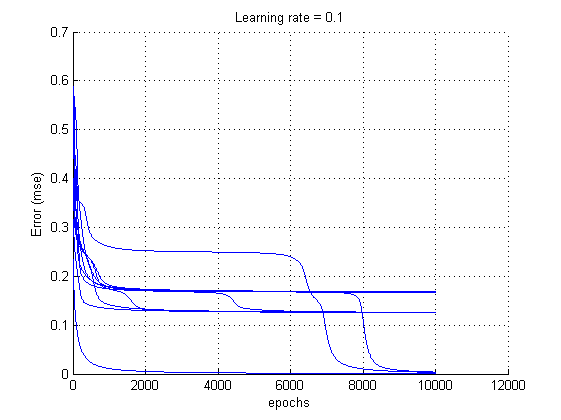
\includegraphics[]{plot2_LR01.png}
	\caption{\label{fig:plot2_LR01}\textbf{Plot 1} from 10 Training sessions with a learning rate of 0.1.}
\end{figure}
\begin{figure}[H] %float here
	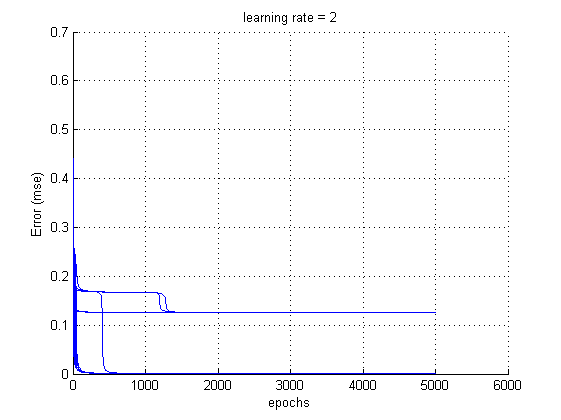
\includegraphics[]{plot2_LR2.png}
	\caption{\label{fig:plot2_LR2}\textbf{Plot 1} from 10 Training sessions with a learning rate of 2.}
\end{figure}
\begin{figure}[H] %float here
	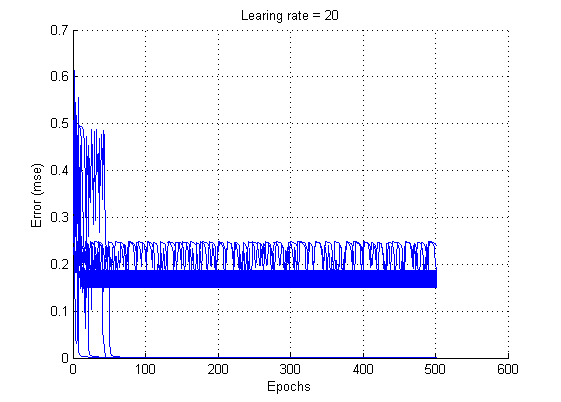
\includegraphics[]{plot2_LR20.png}
	\caption{\label{fig:plot2_LR20}\textbf{Plot 1} from 10 Training sessions with a learning rate of 20.}
\end{figure}
\subsection*{Question 1 \& 2}
Sometimes, as shown in figure \{\ref{fig:plot2_LR01}\}, 
the error plot converges to an value significantly larger than zero.
In these cases the algorithm get's stuck in local minima. If we are taking too 
small steps we and can't get out of small cavities. But we have to be careful: 
a too large learning rate will cause the algorithm to take giant leaps through the landscape. 
Too big steps will make it very hard to find a good solution, and an oscillating 
behaviour is likely to occur; see figure \{\ref{fig:plot2_LR20}\}. 

\begin{figure}[H] %float here
	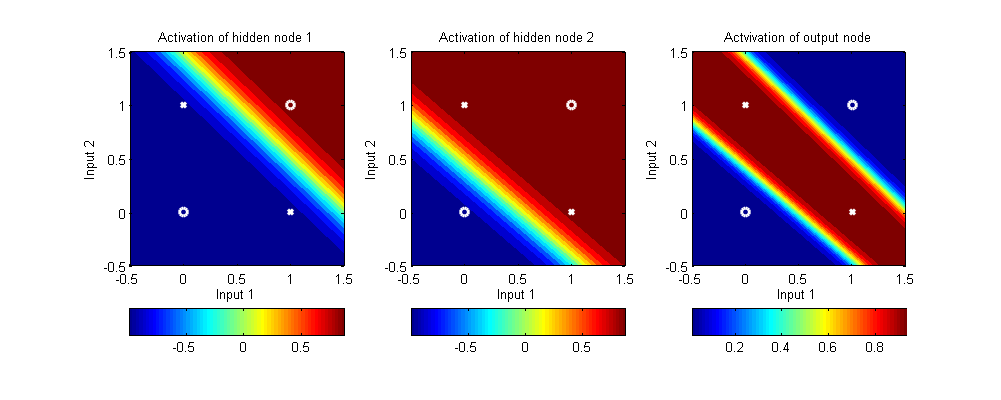
\includegraphics[scale=0.55]{good_bprop_xor_plot.png}
	\caption{\label{fig:good_bprop_xor_plot}\textbf{Plot 2} A good solution found for the XOR problem using back-propagation}
\end{figure}
\begin{figure}[H] %float here
	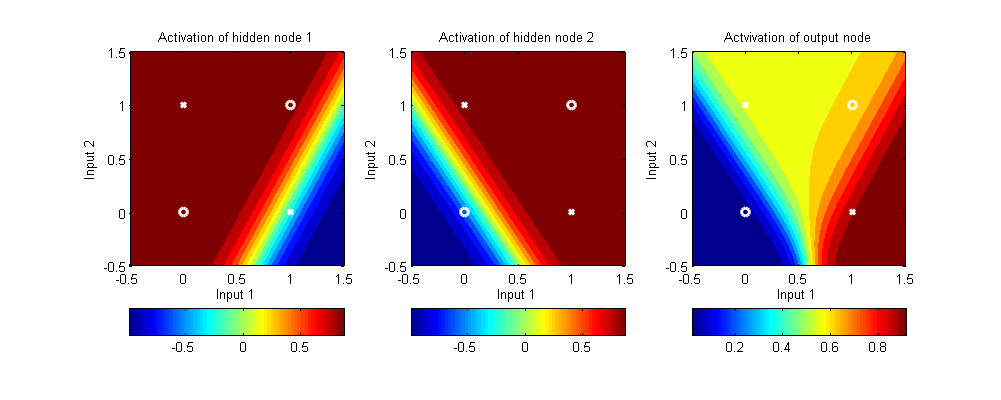
\includegraphics[scale=0.55]{bad_bprop_xor_plot.png}
	\caption{\label{fig:bad_bprop_xor_plot}\textbf{Plot 2} A bad solution found for the XOR problem using back-propagation}
\end{figure}
A visualisation of a well trained network for the XOR problem  
is to plot the result of various values 
as colours, as seen in figure \{\ref{fig:good_bprop_xor_plot}\}. 
Here, we can see the classification of the possible input values. We can 
clearly see the two hyperplanes generated that separates data. 

Here, we also see the hidden node values of possible inputs of the XOR function.
Inspecting the plot ranges of the hidden nodes as well as the output node, we notice that
the range for the hidden nodes are [-1, 1] and the range for the output function is [0, 1].
\subsection*{Question 3}
The reason that the ranges differs is that two 
different sigmoid functions were used as activation functions used for the network. 
For the hidden layer, the hyperbolic tangent function (range [-1, 1]) were used. 
For the output node, the logistic function (range [0, 1]) were used. The authors of 
this report could not find out weather it makes a difference for the algorithm weather 
you use a activation function that ranges from [0, 1] or [-1, 1] but it could be 
convenient if the output activation function has the same range as the actual problem 
output. 
\subsection*{Question 4}
A new neural network gets distributed random weights 
when initialized. The result of this is that the training ends with different 
solutions every time the network is initialized and trained and the 
number of epochs needed to train the network differs as well. 
\subsection*{Question 5}
Consider the coloured plot of the XOR problem 
network nodes (figure \{\ref{fig:good_bprop_xor_plot}\}). We 
know that this plot represents a well trained network and output node is 
representing the boolean XOR function. As for the hidden nodes, study the value 
of the different inputs. For hidden node 1, an input of (0, 0) corresponds to 0 (or 
at least a value very close to zero). $(0, 1)$ also approximates to $0$, $(1, 0) \approx 0$ and 
$(1, 1) \approx 1$. If this node implemented any boolean function it would be the AND function.
In the same way, the hidden node implements the boolean OR function. 
\subsection*{Question 6}
The output node implements the boolean XOR function, 
This is verified in the truth table \{\ref{table:1}\} below. 

\begin{center}
	\label{table:1}
    \begin{tabular} {l | c | r }
        Input & boolean XOR & Network implemented XOR \\
		\hline
        0 0 & 0 & $0.0348 \approx 0$\\
        0 1 & 1 & $0.9744 \approx 1$\\
        1 0 & 1 & $0.9745 \approx 1$\\
        1 1 & 0 & $0.0350 \approx 0$\\
    \end{tabular}
\end{center}

\begin{figure}[H] %float here
	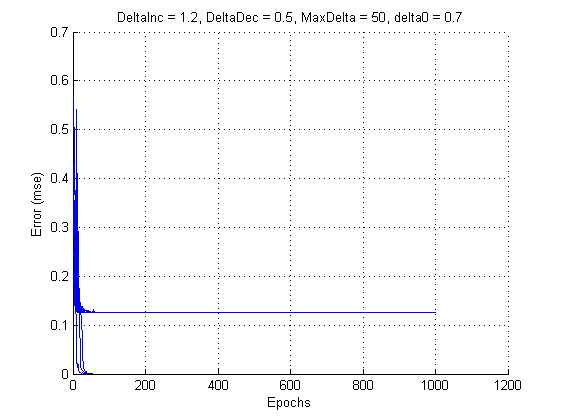
\includegraphics[]{plot3_rprop.png}
	\caption{\label{fig:plot3_rprop}\textbf{Plot 3} Using the Resilient Back-propagation algorithm with the variables: $DeltaInc = 1.2, DeltaDec = 0.5, MaxDelta = 50, delta0 = 0.7$}
\end{figure}
\begin{figure}[H] %float here
	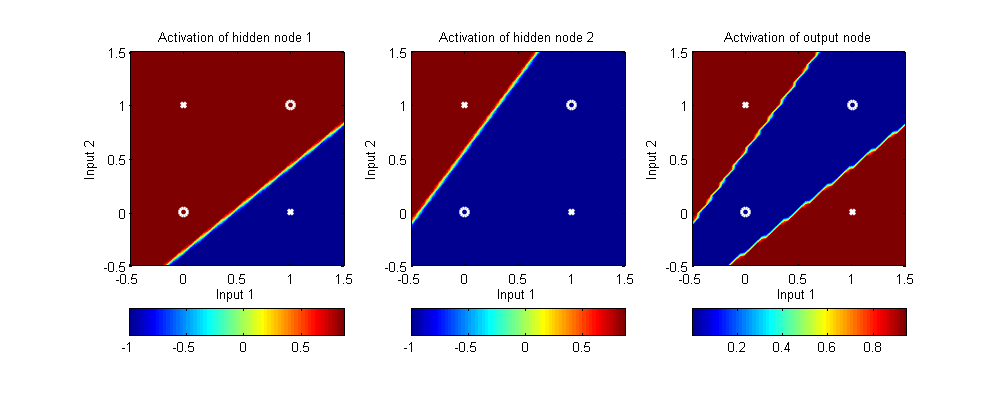
\includegraphics[scale=0.55]{good_rprop_xor_plot.png}
	\caption{\label{fig:good_rprop_xor_plot}\textbf{Plot 3} The plot\_xor of resilient back-propagation.}
\end{figure}
\subsection*{Question 7}
The biggest difference is the difference in number of epochs needed. 
Resilient back propagation needs a lot fewer epoch to reach a minima.
We think that resilient back propagation is better suitable for this problem 
since it finds a minimum in about 400 times less epochs compare to the normal 
back propagation. This is seen in figure \{\ref{fig:plot3_rprop}\}.
A interesting observation from using plot\_xor, seen in figure \{\ref{fig:good_rprop_xor_plot}\} is that the way rprop have classified the groups is a mirrored image of the back-propagation. 

\section{Simple function approximation}
In this task we are trying to approximate the function $f(x) = sin(x) \times sin(5x)$ on the interval $[0, \pi]$ with a MLP. We will use a 10 data points to approximate the function, assuming we don't know it from the start. 
%Insert plot 4 here
\begin{figure}[H] %float here
	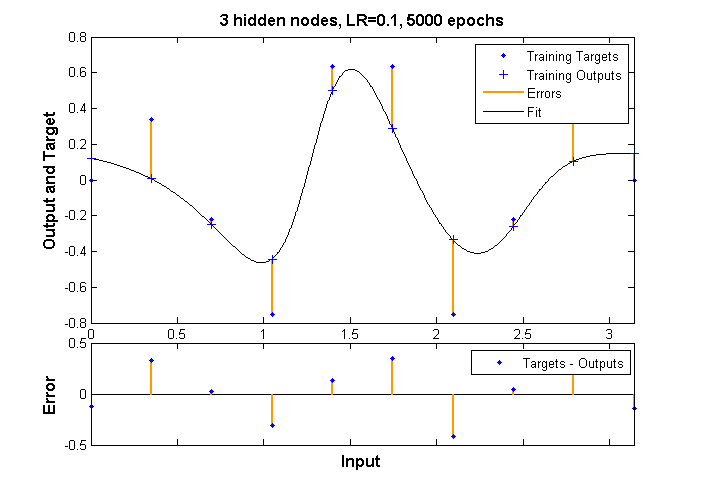
\includegraphics[scale=0.8]{plot4_3nodes.png}
	\caption{\label{fig:plot4_3nodes.png}\textbf{Plot 4} An ANN consisting of 3 nodes with a learning rate of 0.1 for 5000 epochs}
\end{figure}
\begin{figure}[H] %float here
	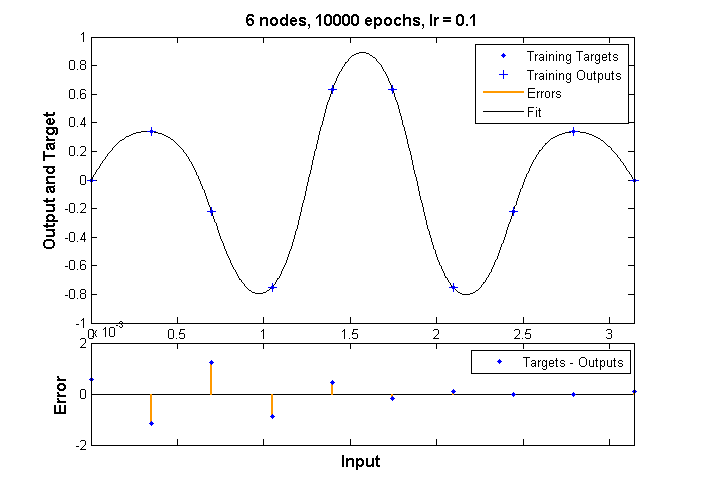
\includegraphics[scale=0.8]{plot4_6nodes.png}
	\caption{\label{fig:plot4_6nodes.png}\textbf{Plot 4} An ANN consisting of 6 nodes with a learning rate of 0.1 for 10000 epochs}
\end{figure}
\begin{figure}[H] %float here
	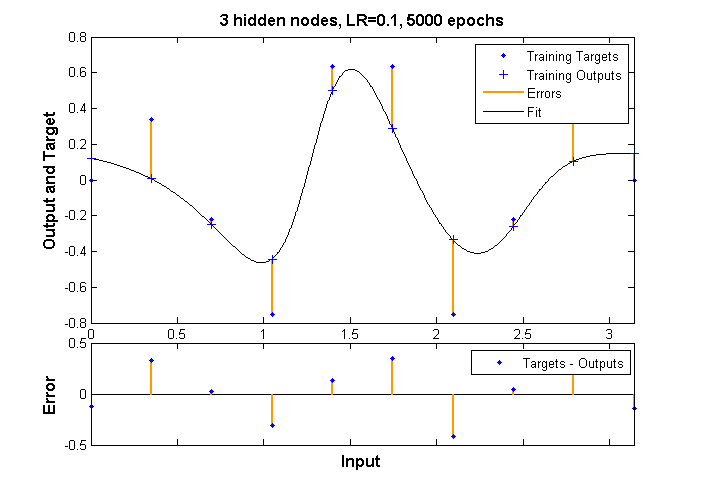
\includegraphics[scale=0.8]{plot4_3nodes.png}
	\caption{\label{fig:plot4_10nodes.png}\textbf{Plot 4} An ANN consisting of 10 nodes with a learning rate of 0.1 for 10000 epochs}
\end{figure}
\begin{figure}[H] %float here
	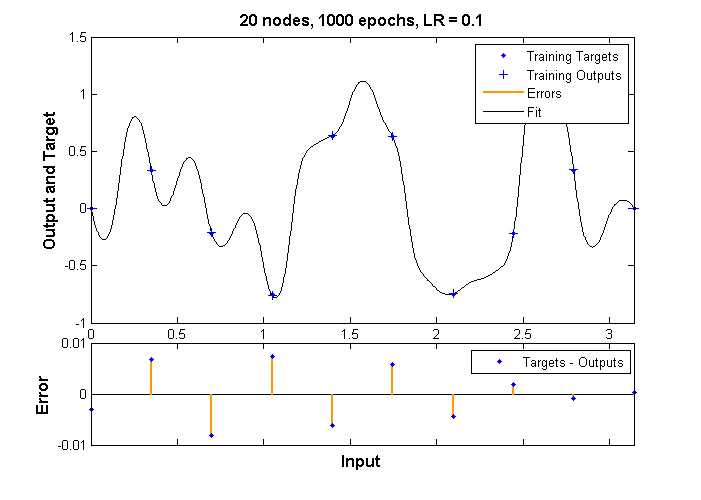
\includegraphics[scale=0.8]{plot4_20nodes.png}
	\caption{\label{fig:plot4_20nodes.png}\textbf{Plot 4} An ANN consisting of 20 nodes with a learning rate of 0.1 for 1000 epochs}
\end{figure}

\subsection*{Question 8}
When using many epochs, we notice that the higher number of nodes we have, the less MSE we get. We suspect that a AAN with more nodes can faster tweak the curve to cross the desired training targets' coordinates since they have more options to optimize the path between the targets. This gives a smaller MSE even though it doesn't necessary mean that it gives us a better answer, an example of this can be seen in the 20 nodes ANN in \{\ref{fig:plot4_20nodes.png}\}, that performance very well in crossing the training targets' coordinates.

\subsection*{Question 9}
The 6 node network, seen in figure \{\ref{fig:plot4_6nodes.png}\} got the approximation that looks most like the desired function. It seems like 3 nodes is not enough to make a plot close to the training targets. This can be seen in figure \{\ref{fig:plot4_3nodes.png}\}. We believe that each node represents a hyper plane and it seems like 3 hyper planes is not enough to plot a curve that crosses the nodes of the actual target data. It seems like the networks with bigger size tend to have to much freedom between the training targets to plot a way towards them. Furthermore the size of 6 nodes seems to limit the shape of the curve between the training target, but express enough freedom to actually cross the target data's coordinates, to represent the desired function. That would as well mean that if we have more target nodes we would benefit if we increase the number of nodes in the network. 
The AAN with 10 nodes, seen in \{\ref{fig:plot4_10nodes.png}\}, shows less freedom of expression between the lines than the 20 node network but a lot more than the 6 node network.

\subsection*{Question 10}
With few hidden nodes we get to few hyper planes to classify the actual target nodes in this problem instance. This is strongly co-related to the number of coordinates the target data express and their location. 

\subsection*{Question 11}
If we have to many hidden nodes, the errors we are testing against is getting less severe, but the approximation towards the function is suffering. There are to many hyperplanes that the AAN can adjust so it's not likely that it will plot it as a smooth curve between the target nodes. Instead it just get rewards for reaching the target nodes, regardless of the angle of the extra  not hyper planes between the target nodes.

\subsection*{Question 12}
We know that the hyperbolic tangent function can only create a few types of hyperplanes, where the most simple is similar to a line. By looking at the desired function we can imagine how many hyperplanes we need to get a good approximation of the function. For every hyperplane we need we should add one hidden node to the MLP. However we need to make sure we have enough nodes in the target data to actually represent this shape.

\subsection*{Question 13}
With resilient back-propagation we get very fast a result that is quite similar to the desired function shape. If we let it run for a long time we don't experience any improvement. If we want more precision we can use normal back propagation but the shape will be more distorted the first iterations but quite fast it will catch up and become better than the resilient back-propagation. The choice is between training time and how close the approximation need to be. 

\section{Classification of wine data}
In this task, we were like in task 1 asked to solve a classification problem. This time 
both the input and the dataset were larger: 178 samples, each with 13
values for the various measurements. Again we do not know 
the relation between the data and the result, 
so we create a NN and leave it to the network to work out a solution for the problem.

\subsection*{Question 14}
As the arity of the input data input grows, 
it both becomes harder to decide the structure of the network and 
choosing the right training parameters. Even though we had difficulties training 
networks 
on this data, we had some success with a 
network trained with the following specifications: The training algorithm was 
resilient back propagation, the network had one hidden layer with 50 
nodes, speed increase 20\% and decrease by 50\%. The network was trained for 
3000 epochs but when training went well, the algorithm usually found a good 
solution in fewer epochs. The confusion matrix 
of one trained network is shown in figure \{\ref{fig:wine_classification}\}. 
As we can see, this network manages to classify 96.6\% of the samples 
into the right class.

\begin{figure}[h!] %float here
    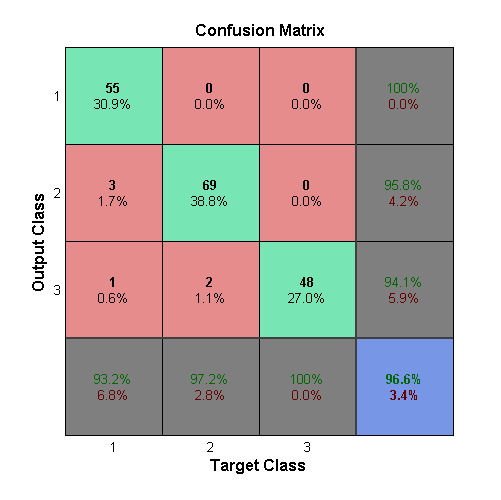
\includegraphics[]{wine_classification.png}
    \caption{\label{fig:wine_classification}Confusion matrix for a successfully trained network for the wine classification problems.}
\end{figure}

\subsection*{Question 15}
Even though the network from the previous subsection had 50 hidden nodes, it was 
still very hard to train. Upon inspecting the distribution of the separate values 
of the input data we notice that some data values are significantly larger 
than others. This results in in big weight shifts for those values 
even if we do not know if that specific 
data is actually more important for determining the class of the 
sample. We made an attempt to solve this problem by 
normalizing the input vector to prevent 
some values to differ a lot from others. 
We experienced great improvement training the same network with the 
normalized input. The 
network now found a solution with very low error every time the network was initialized 
and trained. We had the same success when lowering the number of nodes in the hidden layer, 
and we found that a network with as few as 3 hidden nodes were successful in training on the 
normalized data, and would usually classify all wines into the right class in very 
few $(<50)$ epochs.

\subsection*{Question 16}
Even when having success with normalized data compared to the widely distributed 
data, normalization should be used with caution. The reason is that it discards 
information. As we don't know if certain parameters of the input is more important 
for the classification, we don't know if normalizing can make training harder. 

\section{Task4: Approximating house prices}
In this task we are estimating house prices in Boston based on 506 samples. Each sample contains 13 dimensions with data.
We will split the data into three sets: a training set, a validation set and a test set as an attempt to determine how good the ANN generalizes.

%TODO: insert plot 5 here
\begin{figure}[h!] %float here
	\includegraphics[]{housetraining.png}
	\caption{\label{fig:housetraining}\textbf{Plot 5} House estimate samples run}
\end{figure}

\subsection*{Question 17}
Considering the cases where the algorithm was able to train the network in a significant number of epochs: 
The training set usually has the lowest error rate, since it is the data we use to adjust the weights with. The validation usually has the second lowest error rate. Thus the test set have the highest error rate. The reason the validation data is biased is that even though it is not used to adjust the weights, it is used to select the final model of the network. The test data is the completely unbiased data, which means it usually has the highest error rate. 
In general, even though a network seems to be well trained, it might not perform as good when given fresh data.

\subsection*{Question 18}
In early epochs, the test and validation set is behaving quite randomly. This is because an untrained network starts with a random distribution of the weights. After a while, the curves becomes more smooth. 
After a more significant number of epochs, the validation curve
has minimum after which its error starts to steadily increase. This is the point we know we should stop training in order to prevent over-fitting. 
In the example plot \{\ref{fig:housetraining}\}, we chose the maximum number of epochs where the validation error could increase as 1000, so we continue training for maximum 1000 epochs after we find a minimum in the validation graph. The test set error usually doesn't get much smaller as we train the network for a long time. 

A well trained network should perform well when given fresh data but perhaps the data set was too small or the training method was wrong.

\subsection*{Question 19}
\begin{enumerate}
\item Training the network for a long time does not necessarily mean that it is going to be giving the correct outputs when given inputs outside the training set.

In most cases we have to consider cases where the ANN have to generalize data as it encounters data it haven't trained on.  

\item We need to be careful when deciding when to stop training. Because of the nature of an ANN, having a few failed validation epochs does not mean we already found the optimal solution, so we can't stop training too early. We can also have to be careful to not stop training too late, because that will result in a over-fitted ANN which will perform bad on data that was not in the original training set. 
\end{enumerate}

\section{Task 5: Wrapping up}
\subsection*{Question 20}
We have been considering two different problem, the first is detecting spoiled products at for example a food distribution plant and the second is to detect cancer. There is a tool called electronic nose that can give a representation of smell that a computer can parse. We think this can be used to detect the chemical components that are released in food when it spoils or the chemical components in cancer. We think it would be possible to get enough data for these fields of use to learn an ANN to generalize a patient as cancerous or non-cancerous. This would work well as a complement to human expertise and remove workload from the doctors. 
In food delivery it can be used to early detect spoiled fruit or meat so it can be removed before shipped to the stores.
An interesting observation we made after coming up with this idea is that someone have recently created a machine to detect cancer from the smell. We strongly suspect that that machine is using some kind of machine learning technique.
\end{document}
